\documentclass[12pt,a4paper]{article}

\usepackage{fontspec}
\setmainfont{cmunrm.otf}[
  BoldFont=cmunbx.otf,
  ItalicFont=cmunti.otf,
  BoldItalicFont=cmunbi.otf]
\usepackage[english,russian]{babel}
\usepackage{amsmath,amssymb}
\usepackage{graphicx}
\usepackage{booktabs}
\usepackage{geometry}
\usepackage{caption}
\usepackage{enumitem}
\usepackage{hyperref}
\hypersetup{colorlinks=true,linkcolor=black,citecolor=black,urlcolor=blue}
\geometry{margin=2.5cm}

\captionsetup{font=small,labelfont=bf}
\sloppy

\title{\vspace{-1cm}\Large\bfseries
Естественный язык как целое:\\
выявление сгенерированных текстов на мальтийском языке\\
методами кластеризации и топологического анализа}
\author{Сафонов Матвей\\[2pt]
\small Научный руководитель: проф.\ В.\,А.~Громов\\
\small Национальный исследовательский университет «Высшая школа экономики»}
\date{2026}

\begin{document}
\maketitle

\begin{abstract}
\noindent
Работа выполнена в рамках проекта \emph{Spot the bot} лаборатории В.\,А.~Громова
и посвящена задаче различения текстов, написанных человеком, и текстов,
сгенерированных нейросетевой языковой моделью, для \textbf{мальтийского языка}~--
малоресурсного языка семитской группы. Построен корпус из 36\,452
человеческих текстов, обучена словесная LSTM-модель-генератор, для обоих
корпусов получены облака векторов $n$-грамм на основе SVD-эмбеддингов. Облака
исследованы кластеризацией Уишарта и персистентными гомологиями. Показано,
что облако бот-текстов статистически значимо отличается от человеческого:
оно дробится на большее число кластеров, имеет большую долю шума, хуже
разделено (критерий Дэвиса--Болдина) и топологически сложнее (больше циклов
$H_1$). Различия подтверждены бутстрап-оценкой ($B=40$, критерий
Манна--Уитни, $p<10^{-5}$, размер эффекта Коэна $1{,}2$--$2{,}3$).

\medskip
\noindent\textbf{Ключевые слова:} обработка естественного языка, мальтийский
язык, SVD, латентно-семантическое отображение, LSTM, кластеризация Уишарта,
персистентные гомологии, выявление сгенерированных текстов.
\end{abstract}

\tableofcontents
\newpage

\section{Введение}

Гипотеза о том, что естественный язык представляет собой
\emph{самоорганизованную критическую систему}, развивается в ряде работ
лаборатории В.\,А.~Громова~\cite{gromov2020,gromov2023}. В этой парадигме
текст рассматривается не как линейная последовательность, а как целостный
объект, обладающий геометрической и топологической структурой в пространстве
семантических векторов. Если структура человеческого языка устроена
определённым образом, то текст, порождённый искусственной языковой моделью,
должен отличаться от человеческого именно на уровне этой структуры, даже когда
локально (на уровне отдельных $n$-грамм) он выглядит правдоподобно.

Проект \emph{Spot the bot} ставит задачу проверки этой гипотезы: научиться
\textbf{отличать сгенерированный текст от человеческого} по геометрии облака
его $n$-грамм. Методология проекта применяется к разным языкам; настоящая
работа выполняет полный цикл для \textbf{мальтийского языка} (\texttt{mt}).

Мальтийский интересен как объект исследования: это единственный семитский
язык с латинской письменностью и официальным статусом в ЕС, при этом
малоресурсный~-- готовых нейросетевых моделей и больших корпусов для него
немного. Это делает задачу содержательной и с инженерной стороны.

\paragraph{Цель работы}~-- пройти полный конвейер \emph{Spot the bot} для
мальтийского языка и установить, различимы ли человеческий и сгенерированный
корпуса методами кластеризации и топологического анализа.

\paragraph{Задачи:}
\begin{enumerate}[nosep]
  \item собрать и предобработать корпус мальтийских текстов;
  \item построить словарь SVD-эмбеддингов;
  \item обучить нейросетевой генератор и получить бот-корпус;
  \item сформировать облака векторов $n$-грамм для обоих корпусов;
  \item кластеризовать облака алгоритмом Уишарта и сравнить метрики качества;
  \item исследовать облака методом персистентных гомологий;
  \item оценить статистическую значимость различий.
\end{enumerate}

\section{Постановка задачи}

Пусть дан корпус человеческих текстов $\mathcal{H}$ и корпус
сгенерированных текстов $\mathcal{B}$ сопоставимого объёма. Каждое слово
отображается в вектор фиксированной размерности $m$; $n$ подряд идущих слов
дают вектор $n$-граммы размерности $n\cdot m$ (конкатенация). Множество всех
$n$-грамм корпуса образует \emph{облако точек} в $\mathbb{R}^{nm}$.

Формально требуется проверить нулевую гипотезу
\[
  H_0:\quad \text{облака }\;\mathcal{H}\;\text{и}\;\mathcal{B}\;
  \text{статистически неразличимы по структурным характеристикам,}
\]
против альтернативы $H_1$ об их различии. В качестве структурных
характеристик берутся: число и размеры кластеров и метрики качества
кластеризации (внутренние меры валидности, гл.~23~\cite{aggarwal2013}), а
также топологические инварианты~-- числа Бетти и характеристики диаграмм
персистентности.

\section{Теоретические основы}

\subsection{SVD-эмбеддинги и латентно-семантическое отображение}

Основной тип эмбеддингов в методологии проекта~-- эмбеддинги на основе
сингулярного разложения, восходящие к латентно-семантическому отображению
Беллегарда~\cite{bellegarda2005}. По очищенному корпусу строится
взвешенная матрица «термин--документ» $A\in\mathbb{R}^{V\times D}$
($V$~-- число уникальных слов, $D$~-- число текстов) с весами TF-IDF.
Усечённое сингулярное разложение ранга $k$
\[
  A \;\approx\; U_k\,\Sigma_k\,V_k^{\top},\qquad
  U_k\in\mathbb{R}^{V\times k},\;\;
  \Sigma_k=\operatorname{diag}(\sigma_1,\dots,\sigma_k),
\]
даёт векторное представление слова: $i$-й строке $U_k\Sigma_k$
соответствует $k$-мерный вектор $i$-го слова. Существенное свойство метода:
для получения эмбеддинга меньшей размерности $d<k$ повторное разложение не
нужно~-- достаточно взять первые $d$ компонент вектора. Поэтому разложение
проводится один раз с большим $k$ (здесь $k=1024$).

\subsection{Кластеризация Уишарта}

Алгоритм Уишарта~\cite{wishart1969}~-- плотностный метод кластеризации
(\emph{mode analysis}), выделяющий кластеры как области высокой плотности,
разделённые областями низкой плотности. Плотность в точке $x_i$ оценивается
по расстоянию $r_k(i)$ до её $k$-го ближайшего соседа:
\[
  p(x_i) \;=\; \frac{k}{n\cdot V_d\cdot r_k(i)^{\,d}},
  \qquad
  V_d=\frac{\pi^{d/2}}{\Gamma(d/2+1)},
\]
где $n$~-- число точек, $d$~-- размерность, $V_d$~-- объём единичного
$d$-мерного шара. Точки обрабатываются в порядке убывания плотности; для
очередной точки по графу $k$ ближайших соседей определяются уже
обработанные кластеры, с которыми она связана:
\begin{itemize}[nosep]
  \item связей нет~-- образуется новый кластер;
  \item один кластер~-- точка присоединяется к нему (если он не «завершён»);
  \item несколько кластеров~-- \emph{значимые} кластеры (с перепадом
        плотности $\ge h$) замораживаются, точка уходит в шум; незначимые
        кластеры сливаются.
\end{itemize}
Параметрами алгоритма являются $k$ (число соседей для оценки плотности) и
$h$ (порог значимости). Качество полученной кластеризации оценивается
внутренними мерами валидности (гл.~23~\cite{aggarwal2013}): силуэт,
индекс Дэвиса--Болдина, индекс Калинского--Харабаса.

\subsection{Персистентные гомологии}

Персистентные гомологии~\cite{edelsbrunner2010,zhu2013}~-- инструмент
топологического анализа данных. По облаку точек строится фильтрация
комплексов Виеториса--Рипса: при росте параметра $\varepsilon$ точки,
оказавшиеся на расстоянии $\le\varepsilon$, соединяются ребрами, образуются
симплексы. В ходе фильтрации топологические особенности
($H_0$~-- связные компоненты, $H_1$~-- одномерные циклы) «рождаются» и
«умирают». Диаграмма персистентности фиксирует пары (рождение, смерть);
долго живущие особенности считаются значимыми, короткоживущие~-- шумом.
Числовые характеристики: числа Бетти $b_0,b_1$, суммарная и максимальная
персистентность, энтропия персистентности
\[
  E=-\sum_i \frac{\ell_i}{L}\,\log\frac{\ell_i}{L},
  \qquad \ell_i\;-\;\text{время жизни}\;i\text{-й особенности},\;\;
  L=\sum_i\ell_i.
\]

\section{Сбор и предобработка корпуса}

\subsection{Источники}

Корпус мальтийских текстов собран из открытых источников
(см.~табл.~\ref{tab:corpus}): академический корпус Мальтийского университета
(MLRS / Korpus Malti), репозиторий научных работ UM, мальтийская Википедия,
блоги и пресса, нехудожественные тексты. Всего собрано свыше 110~тыс.\ сырых
текстовых файлов; для балансировки источников блоги и пресса ограничены до
8\,000 текстов каждый.

\begin{table}[ht]
\centering
\caption{Состав человеческого корпуса после балансировки источников}
\label{tab:corpus}
\begin{tabular}{lr}
\toprule
Источник & Число текстов \\
\midrule
Репозиторий научных работ UM (\texttt{umlib\_oar}) & 11\,280 \\
Блоги (\texttt{blogs}) & 8\,000 \\
Пресса (\texttt{press\_mt}) & 8\,000 \\
Википедия (\texttt{wiki}) & 7\,041 \\
Нехудожественные тексты (\texttt{nonfiction}) & 2\,113 \\
Дипломные работы (\texttt{theses}) & 18 \\
\midrule
\textbf{Итого} & \textbf{36\,452} \\
\bottomrule
\end{tabular}
\end{table}

\subsection{Предобработка}

Предобработка приводит словоформы к начальной форме (лемматизация) и заменяет
служебные части речи специальными токенами: местоимения~-- на \texttt{PRON1},
числительные~-- на \texttt{ORDINAL1}, имена собственные~-- на \texttt{PERSON1};
пунктуация и символы отбрасываются. Замены опираются на часть речи, поэтому
лемматизатору необходима POS-разметка.

\paragraph{Три варианта лемматизации.} Поскольку мальтийский малоресурсен и
готового надёжного лемматизатора для него нет, реализованы и сопоставлены три
варианта:
\begin{itemize}[nosep]
  \item \texttt{L1}~-- нейросетевой лемматизатор \texttt{Stanza} (конвейер
        \texttt{tokenize\,/\,pos\,/\,lemma}). POS-разметка надёжна, но
        нейролеммы для малоресурсного языка часто неточны и лексически ничем
        не подкреплены.
  \item \texttt{L3}~-- чисто правиловый препроцессор без NLP-библиотек
        (стрипперы мальтийских аффиксов: артикли с дефисом \texttt{il-},
        \texttt{it-}, \ldots, проклитики с апострофом \texttt{b'},
        \texttt{f'}, \ldots, притяжательные и объектные суффиксы), по духу
        близкий лемматизатору Субхангулова для татарского. «Строгий по
        методике», но не даёт частей речи, поэтому служебные замены
        выполняются лишь эвристически (по спискам и регистру), а не по
        реальной POS.
  \item \texttt{L2}~-- комбинированный: POS-разметка и базовая лемма берутся
        из \texttt{Stanza}, после чего применяется собственный
        \emph{лексиконный} лемматизатор на основе морфологической базы
        мальтийского Ġabra (1\,303\,378 словоформ).
\end{itemize}

\paragraph{Как устроен лемматизатор L2.} Для каждой словоформы $w$ (если её
часть речи не служебная и не отбрасывается) лемма определяется каскадом
поисков по таблице Ġabra; первый сработавший шаг даёт результат:
\begin{enumerate}[nosep]
  \item точный поиск $w$ (в нижнем регистре) в Ġabra;
  \item поиск формы со снятыми диакритиками (\texttt{ċġħż}$\to$\texttt{cghz});
  \item поиск после отсечения артикля/проклитики
        (\texttt{il-}, \texttt{b'}, \ldots), в том числе без диакритик;
  \item откат на лемму, предложенную \texttt{Stanza};
  \item если ничего не найдено~-- сама исходная словоформа.
\end{enumerate}
Тем самым L2 объединяет сильные стороны L1 и L3: достоверную POS-разметку для
служебных замен~-- и точную, лексически выверенную лемму вместо ненадёжной
нейросетевой. Распределение источников итоговых лемм по корпусу: Ġabra~--
$\approx4{,}1\,\%$ токенов (исправление формы), нейролемма \texttt{Stanza}~--
$<0{,}1\,\%$, остальные $\approx95{,}9\,\%$ совпадают с исходной формой (слово
уже в начальной форме или отсутствует в Ġabra). Низкая доля собственно
изменённых токенов отражает аналитичность корпуса и пределы покрытия лексикона
для малоресурсного языка.

\paragraph{Выбор варианта.} В качестве рабочего выбран \texttt{L2}: он даёт
наиболее точные именно мальтийские леммы при сохранении требуемых методикой
POS-замен, тогда как \texttt{L1} лексически слабее, а \texttt{L3} теряет
информацию о частях речи. Весь дальнейший конвейер (SVD-словарь, генератор,
$n$-граммы, кластеризация, топология) построен на корпусе \texttt{L2}. Итог:
36\,452 очищенных текста, около 39{,}3~млн словоупотреблений; на выходе~--
единый файл, одна строка~-- один текст.

\section{Построение эмбеддингов}

\subsection{SVD-словарь}

По очищенному корпусу с помощью \texttt{TfidfVectorizer} построена матрица
«термин--документ». В качестве \texttt{token\_pattern} задан мальтийский
алфавит (включая буквы «ċ, ġ, ħ, ż»), цифры, дефис и
апостроф~-- это отсекает пунктуацию и иноязычные вкрапления. Получена
разреженная матрица размера $93\,343\times36\,452$ (плотность $0{,}0032$).

К матрице применено усечённое сингулярное разложение ранга $k=1024$.
Сингулярные значения убывают от $\sigma_1\approx39{,}7$ до
$\sigma_{1024}\approx2{,}3$. Результат~-- словарь
$\{\text{слово}\mapsto\text{вектор}\in\mathbb{R}^{1024}\}$ для 93\,343 слов.

\subsection{word2vec}

Для сравнения построены также эмбеддинги word2vec (CBOW и Skip-gram,
размерность 100, окно 5) на том же корпусе средствами \texttt{gensim}
(словарь~-- 107\,405 слов).

\section{Генерация бот-корпуса}

Бот-корпус порождается нейросетевым генератором, обученным на человеческом
корпусе. Использована \textbf{словесная LSTM} языковая модель: она оперирует
теми же лемма-токенами, что и SVD-словарь, поэтому сгенерированные тексты
напрямую пригодны для построения $n$-грамм.

\paragraph{Архитектура и обучение.} Модель: слой эмбеддинга (300),
двухслойная LSTM (скрытый размер 512, dropout $0{,}3$), линейный слой на
словарь (50\,000 наиболее частотных слов); всего $44{,}4$~млн параметров.
Обучение~-- предсказание следующего токена с усечённым BPTT, оптимизатор
Adam, 8 эпох. Перплексия на отложенной выборке снизилась со 164 (эпоха~1) до
\textbf{98} (эпоха~8).

\paragraph{Генерация.} Из обученной модели сгенерировано 36\,452 текста~--
столько же, сколько в человеческом корпусе. Длина каждого текста берётся из
эмпирического распределения длин человеческих текстов, что обеспечивает
сопоставимость корпусов по объёму. Итоговый бот-корпус: 36\,452 текста,
$29{,}6$~млн токенов.

\section{Датасет $n$-грамм}

Для каждого корпуса скользящим окном длины $n$ выделяются $n$-граммы; вектор
каждого слова берётся из SVD-словаря (первые $m$ компонент), векторы слов
$n$-граммы конкатенируются в вектор размерности $n\cdot m$. Если хотя бы одно
слово $n$-граммы отсутствует в словаре, $n$-грамма пропускается.

Облака формировались для нескольких конфигураций $(n,m)$; в каждом облаке~--
по 300\,000 векторов $n$-грамм для человека и для бота. Доля пропущенных
из-за отсутствия слова в словаре $n$-грамм растёт с $n$ (для $n=3$~-- около
20\,\%, для $n=5$~-- свыше 95\,\%), что естественно: вероятность того, что
\emph{все} слова длинной $n$-граммы есть в словаре, падает с ростом $n$.

\section{Кластеризация Уишарта: эксперименты}

\subsection{Свип параметров}

Сначала исследована чувствительность алгоритма к параметрам $k$ и $h$ на
конфигурации $n=4,\;m=8$. Параметр значимости $h$ оказался практически
инертным: при изменении от $0{,}2$ до $125$ результаты не менялись~--
в высокоразмерном облаке перепады плотности внутри кластеров намного
превосходят любое разумное $h$. Параметр $k$, напротив, сильно влияет на
дробность разбиения: $k=7$ даёт около 400 кластеров, $k=51$~-- около 30.
Доля шума при любых параметрах высока (75--87\,\%)~-- это структурное
свойство плотностной кластеризации в пространстве высокой размерности.
Для дальнейших экспериментов зафиксированы $k=11,\;h=1$.

\subsection{Сравнение конфигураций}

Сопоставлены 6 конфигураций (тип эмбеддинга $\times$ параметры $n,m$),
табл.~\ref{tab:configs}. Во \emph{всех} конфигурациях облако бота дробится на
\emph{большее} число кластеров, чем человеческое
($\Delta_{\text{кл}}=+13\ldots+31$). Эмбеддинги word2vec при срезе до 8
компонент кластеризуются вырожденно (силуэт уходит в отрицательную область),
что подтверждает уместность именно SVD-эмбеддингов. Наилучшее расхождение
human/bot по совокупности метрик даёт конфигурация \textbf{SVD, $n=4$,
$m=16$}.

\begin{table}[ht]
\centering
\caption{Сравнение конфигураций (Уишарт, $k=11$, $h=1$, по 30\,000 $n$-грамм).
H~-- человек, B~-- бот}
\label{tab:configs}
\small
\begin{tabular}{llrr rr rr r}
\toprule
Эмб. & $(n,m)$ & dim & H кл. & B кл. & H шум & B шум & $\Delta$ кл. \\
\midrule
SVD  & $(3,8)$  & 24  & 321 & 352 & 64{,}2\,\% & 65{,}1\,\% & $+31$ \\
SVD  & $(4,8)$  & 32  & 234 & 247 & 77{,}9\,\% & 79{,}4\,\% & $+13$ \\
SVD  & $(5,8)$  & 40  & 156 & 169 & 84{,}6\,\% & 83{,}6\,\% & $+13$ \\
SVD  & $(4,16)$ & 64  & 273 & 302 & 71{,}2\,\% & 75{,}1\,\% & $+29$ \\
SVD  & $(4,32)$ & 128 & 305 & 322 & 62{,}8\,\% & 64{,}3\,\% & $+17$ \\
word2vec & $(4,8)$ & 32 & 17 & 30 & 93{,}5\,\% & 92{,}6\,\% & $+13$ \\
\bottomrule
\end{tabular}
\end{table}

\subsection{Финальная конфигурация}

Полный анализ на конфигурации SVD, $n=4$, $m=16$ (табл.~\ref{tab:final})
показывает: бот-облако имеет больше кластеров, больше шума, выше индекс
Дэвиса--Болдина (хуже разделено) и выше индекс Калинского--Харабаса; при этом
крупнейший кластер у человека больше~-- человеческое облако имеет более
выраженное плотное ядро. Распределение размеров кластеров приведено на
рис.~\ref{fig:wishart}.

\begin{table}[ht]
\centering
\caption{Кластеризация Уишарта, конфигурация SVD $n{=}4,\,m{=}16$}
\label{tab:final}
\begin{tabular}{lrr}
\toprule
Метрика & Человек & Бот \\
\midrule
Число кластеров        & 275   & 293 \\
Доля шума              & 72{,}0\,\% & 72{,}5\,\% \\
Силуэт                 & 0{,}359 & 0{,}366 \\
Индекс Дэвиса--Болдина & 0{,}953 & 1{,}158 \\
Индекс Калинского--Харабаса & 235 & 329 \\
Крупнейший кластер     & 1{,}82\,\% & 1{,}64\,\% \\
\bottomrule
\end{tabular}
\end{table}

\begin{figure}[ht]
\centering
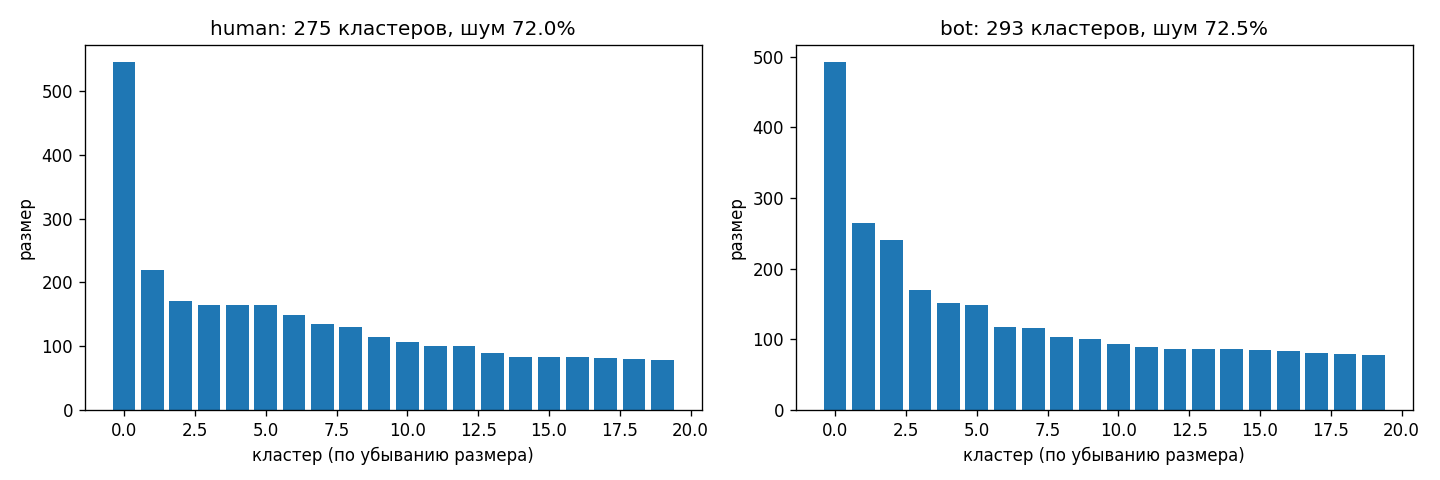
\includegraphics[width=\textwidth]{figures/wishart_sizes.png}
\caption{Распределение размеров кластеров (по убыванию) для человеческого и
бот-облака, конфигурация SVD $n{=}4,\,m{=}16$.}
\label{fig:wishart}
\end{figure}

\subsection{Оценка статистической значимости}

Чтобы убедиться, что различия не являются артефактом конкретной подвыборки,
проведена бутстрап-оценка: $B=40$ раз бралась новая независимая подвыборка по
30\,000 $n$-грамм для человека и для бота, для каждой считалась кластеризация
Уишарта. Поскольку подвыборки человека и бота независимы, применялся
\emph{двухвыборочный} критерий Манна--Уитни; доверительный интервал строился
для \emph{среднего} различия $\Delta=\overline{x}_B-\overline{x}_H$ через
стандартную ошибку, размер эффекта~-- $d$ Коэна.

\begin{table}[ht]
\centering
\caption{Значимость различий (бутстрап $B=40$, SVD $n{=}4,\,m{=}16$).
Звёздочкой отмечены значимые метрики ($p<0{,}05$, ДИ не включает 0)}
\label{tab:boot}
\small
\resizebox{\textwidth}{!}{%
\begin{tabular}{lrrrl rr}
\toprule
Метрика & Человек & Бот & $\Delta$ & 95\,\% ДИ $\Delta$ & $p$ & $d$ \\
\midrule
Число кластеров       & $276{,}2\pm8{,}3$ & $289{,}1\pm10{,}1$ & $+12{,}9$ & $[8{,}9;\,16{,}9]$ & $5\!\cdot\!10^{-7}$ & $1{,}40^{*}$ \\
Доля шума             & $0{,}709\pm0{,}010$ & $0{,}730\pm0{,}009$ & $+0{,}021$ & $[0{,}017;\,0{,}026]$ & $3\!\cdot\!10^{-12}$ & $2{,}27^{*}$ \\
Дэвис--Болдин         & $1{,}001\pm0{,}087$ & $1{,}144\pm0{,}138$ & $+0{,}143$ & $[0{,}093;\,0{,}194]$ & $3\!\cdot\!10^{-6}$ & $1{,}25^{*}$ \\
Калинский--Харабас    & $278{,}8\pm38{,}4$ & $348{,}9\pm74{,}3$ & $+70{,}1$ & $[44;\,96]$ & $2\!\cdot\!10^{-6}$ & $1{,}19^{*}$ \\
Силуэт                & $0{,}355\pm0{,}012$ & $0{,}361\pm0{,}015$ & $+0{,}006$ & $[-0{,}000;\,0{,}012]$ & $0{,}081$ & $0{,}41$ \\
\bottomrule
\end{tabular}}
\end{table}

Результат (табл.~\ref{tab:boot}): \textbf{4 из 5 метрик различают человека и
бота статистически значимо} ($p<10^{-5}$, размер эффекта Коэна
$1{,}2$--$2{,}3$~-- большой). Незначима лишь метрика силуэта~-- этим
объясняется, почему её знак «плавал» от конфигурации к конфигурации.

\section{Топологический анализ}

К облакам человека и бота (конфигурация SVD $n{=}4,\,m{=}16$) применены
персистентные гомологии: для устойчивости результат усреднён по 5 подвыборкам
по 2\,000 точек, размерность гомологий~-- до $H_1$. Результаты~--
табл.~\ref{tab:topo}, диаграммы персистентности~-- рис.~\ref{fig:topo}.

\begin{table}[ht]
\centering
\caption{Топологические характеристики облаков (среднее $\pm$ ст.\ откл.\ по
5 подвыборкам)}
\label{tab:topo}
\begin{tabular}{lrr}
\toprule
Характеристика & Человек & Бот \\
\midrule
$H_0$, число Бетти & $1997\pm2$ & $1995\pm3$ \\
$H_1$, число Бетти (циклы) & $1012\pm21$ & $1105\pm28$ \\
$H_1$, суммарная персистентность & $128{,}9$ & $158{,}5$ \\
$H_1$, энтропия персистентности & $6{,}41$ & $6{,}42$ \\
\bottomrule
\end{tabular}
\end{table}

\begin{figure}[ht]
\centering
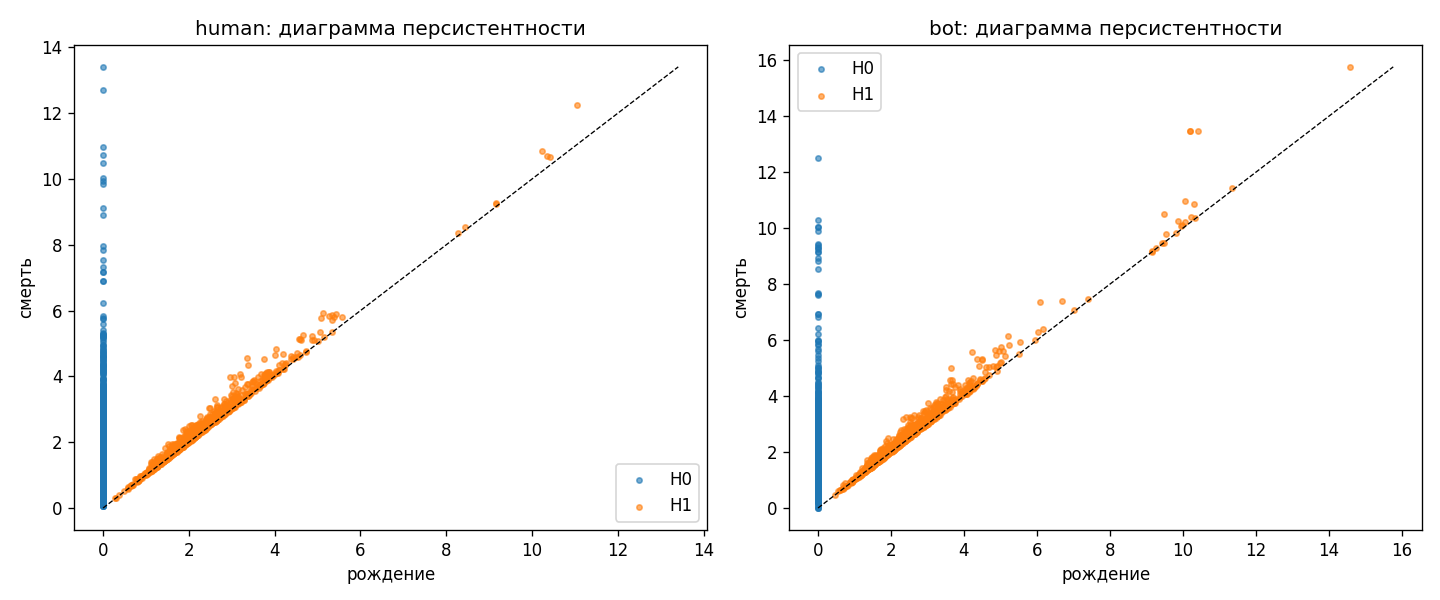
\includegraphics[width=\textwidth]{figures/persistence_diagrams.png}
\caption{Диаграммы персистентности человеческого и бот-облака
(конфигурация SVD $n{=}4,\,m{=}16$).}
\label{fig:topo}
\end{figure}

Облако бота содержит примерно на 93 цикла $H_1$ больше и обладает большей
суммарной персистентностью одномерных особенностей. С учётом разброса по
подвыборкам это различие также значимо (приближённый 95\,\% ДИ для разности
$\approx[62;\,124]$). Топологический вывод согласуется с результатом
кластеризации: облако бота \emph{сложнее} и \emph{раздробленнее}.

\section{Обсуждение}

Два независимых метода~-- плотностная кластеризация и топологический
анализ~-- дают согласованный результат. Человеческое облако $n$-грамм
\textbf{консолидированнее}: меньше кластеров, выраженное плотное ядро
(больший крупнейший кластер), меньше топологических циклов. Облако бота
\textbf{раздробленнее и топологически сложнее}: больше кластеров, выше доля
шума, хуже разделение кластеров, больше циклов $H_1$.

Содержательно это можно интерпретировать так: словесная LSTM, обучаясь
предсказывать следующее слово, хорошо воспроизводит \emph{локальную}
сочетаемость, но не воспроизводит \emph{глобальную} организацию
семантического пространства~-- человеческий текст «стягивается» к
устойчивому ядру тем и конструкций, тогда как сгенерированный
расползается на множество мелких, плохо разделённых сгустков.

\paragraph{Ограничения.} Доля шума в кластеризации высока (около 72\,\%)~--
следствие проклятия размерности; абсолютные значения метрик нужно
трактовать с осторожностью, тогда как \emph{различия} между корпусами
устойчивы и значимы. Параметр значимости $h$ алгоритма Уишарта в
высокоразмерном пространстве оказался неинформативен. Эмбеддинги word2vec
при наивном срезе компонент непригодны~-- требуется отдельная адаптация.

\paragraph{Направления развития.} Имеет смысл: исследовать влияние
температуры генерации и качества LSTM на различимость; сравнить с другими
архитектурами генератора; применить нормировку признаков перед
кластеризацией; расширить топологический анализ до $H_2$ и до
сравнения диаграмм метрикой Вассерштейна.

\section{Заключение}

В работе пройден полный конвейер проекта \emph{Spot the bot} для
мальтийского языка: собран и предобработан корпус из 36\,452 текстов,
построен SVD-словарь ($93\,343\times1024$), обучена словесная
LSTM-модель-генератор (перплексия 98) и порождён бот-корпус
сопоставимого объёма, сформированы облака $n$-грамм, проведены кластеризация
Уишарта и топологический анализ.

\textbf{Главный результат:} человеческий и сгенерированный корпуса
\emph{статистически значимо различимы} по структуре облака $n$-грамм. Четыре
из пяти метрик кластеризации различают их с $p<10^{-5}$ и большим размером
эффекта; топологический анализ независимо подтверждает: бот-облако содержит
больше одномерных циклов. Тем самым для мальтийского языка подтверждается
исходная гипотеза проекта: сгенерированный текст отличается от
человеческого на уровне целостной геометрической и топологической
структуры.

\begin{thebibliography}{9}
\bibitem{gromov2020} Gromov V.\,A., Migrina A.\,M.
  A Language as a Self-Organized Critical System~// Complexity, 2020.
\bibitem{gromov2023} Gromov V.\,A., Dang Q.\,N.
  Semantic and Sentiment Trajectories of Literary Texts~// 2023.
\bibitem{bellegarda2005} Bellegarda J.\,R.
  Latent Semantic Mapping~// IEEE Signal Processing Magazine, 2005.
\bibitem{wishart1969} Wishart D.
  Mode Analysis: A Generalization of Nearest Neighbour which Reduces
  Chaining Effects~// Numerical Taxonomy, 1969.
\bibitem{aggarwal2013} Aggarwal C.\,C., Reddy C.\,K. (eds.)
  Data Clustering: Algorithms and Applications.~-- CRC Press, 2013.~--
  Гл.~23: Cluster Validation Measures.
\bibitem{edelsbrunner2010} Edelsbrunner H., Harer J.
  Computational Topology: An Introduction.~-- AMS, 2010.
\bibitem{zhu2013} Zhu X.
  Persistent Homology: An Introduction and a New Text Representation for
  Natural Language Processing~// IJCAI, 2013.
\end{thebibliography}

\end{document}
